\documentclass[]{article}
\usepackage{lmodern}
\usepackage{amssymb,amsmath}
\usepackage{ifxetex,ifluatex}
\usepackage{fixltx2e} % provides \textsubscript
\ifnum 0\ifxetex 1\fi\ifluatex 1\fi=0 % if pdftex
  \usepackage[T1]{fontenc}
  \usepackage[utf8]{inputenc}
\else % if luatex or xelatex
  \ifxetex
    \usepackage{mathspec}
  \else
    \usepackage{fontspec}
  \fi
  \defaultfontfeatures{Ligatures=TeX,Scale=MatchLowercase}
\fi
% use upquote if available, for straight quotes in verbatim environments
\IfFileExists{upquote.sty}{\usepackage{upquote}}{}
% use microtype if available
\IfFileExists{microtype.sty}{%
\usepackage{microtype}
\UseMicrotypeSet[protrusion]{basicmath} % disable protrusion for tt fonts
}{}
\usepackage[margin=1in]{geometry}
\usepackage{hyperref}
\hypersetup{unicode=true,
            pdftitle={Statistical Inference},
            pdfauthor={Sandesh},
            pdfborder={0 0 0},
            breaklinks=true}
\urlstyle{same}  % don't use monospace font for urls
\usepackage{color}
\usepackage{fancyvrb}
\newcommand{\VerbBar}{|}
\newcommand{\VERB}{\Verb[commandchars=\\\{\}]}
\DefineVerbatimEnvironment{Highlighting}{Verbatim}{commandchars=\\\{\}}
% Add ',fontsize=\small' for more characters per line
\usepackage{framed}
\definecolor{shadecolor}{RGB}{248,248,248}
\newenvironment{Shaded}{\begin{snugshade}}{\end{snugshade}}
\newcommand{\AlertTok}[1]{\textcolor[rgb]{0.94,0.16,0.16}{#1}}
\newcommand{\AnnotationTok}[1]{\textcolor[rgb]{0.56,0.35,0.01}{\textbf{\textit{#1}}}}
\newcommand{\AttributeTok}[1]{\textcolor[rgb]{0.77,0.63,0.00}{#1}}
\newcommand{\BaseNTok}[1]{\textcolor[rgb]{0.00,0.00,0.81}{#1}}
\newcommand{\BuiltInTok}[1]{#1}
\newcommand{\CharTok}[1]{\textcolor[rgb]{0.31,0.60,0.02}{#1}}
\newcommand{\CommentTok}[1]{\textcolor[rgb]{0.56,0.35,0.01}{\textit{#1}}}
\newcommand{\CommentVarTok}[1]{\textcolor[rgb]{0.56,0.35,0.01}{\textbf{\textit{#1}}}}
\newcommand{\ConstantTok}[1]{\textcolor[rgb]{0.00,0.00,0.00}{#1}}
\newcommand{\ControlFlowTok}[1]{\textcolor[rgb]{0.13,0.29,0.53}{\textbf{#1}}}
\newcommand{\DataTypeTok}[1]{\textcolor[rgb]{0.13,0.29,0.53}{#1}}
\newcommand{\DecValTok}[1]{\textcolor[rgb]{0.00,0.00,0.81}{#1}}
\newcommand{\DocumentationTok}[1]{\textcolor[rgb]{0.56,0.35,0.01}{\textbf{\textit{#1}}}}
\newcommand{\ErrorTok}[1]{\textcolor[rgb]{0.64,0.00,0.00}{\textbf{#1}}}
\newcommand{\ExtensionTok}[1]{#1}
\newcommand{\FloatTok}[1]{\textcolor[rgb]{0.00,0.00,0.81}{#1}}
\newcommand{\FunctionTok}[1]{\textcolor[rgb]{0.00,0.00,0.00}{#1}}
\newcommand{\ImportTok}[1]{#1}
\newcommand{\InformationTok}[1]{\textcolor[rgb]{0.56,0.35,0.01}{\textbf{\textit{#1}}}}
\newcommand{\KeywordTok}[1]{\textcolor[rgb]{0.13,0.29,0.53}{\textbf{#1}}}
\newcommand{\NormalTok}[1]{#1}
\newcommand{\OperatorTok}[1]{\textcolor[rgb]{0.81,0.36,0.00}{\textbf{#1}}}
\newcommand{\OtherTok}[1]{\textcolor[rgb]{0.56,0.35,0.01}{#1}}
\newcommand{\PreprocessorTok}[1]{\textcolor[rgb]{0.56,0.35,0.01}{\textit{#1}}}
\newcommand{\RegionMarkerTok}[1]{#1}
\newcommand{\SpecialCharTok}[1]{\textcolor[rgb]{0.00,0.00,0.00}{#1}}
\newcommand{\SpecialStringTok}[1]{\textcolor[rgb]{0.31,0.60,0.02}{#1}}
\newcommand{\StringTok}[1]{\textcolor[rgb]{0.31,0.60,0.02}{#1}}
\newcommand{\VariableTok}[1]{\textcolor[rgb]{0.00,0.00,0.00}{#1}}
\newcommand{\VerbatimStringTok}[1]{\textcolor[rgb]{0.31,0.60,0.02}{#1}}
\newcommand{\WarningTok}[1]{\textcolor[rgb]{0.56,0.35,0.01}{\textbf{\textit{#1}}}}
\usepackage{graphicx,grffile}
\makeatletter
\def\maxwidth{\ifdim\Gin@nat@width>\linewidth\linewidth\else\Gin@nat@width\fi}
\def\maxheight{\ifdim\Gin@nat@height>\textheight\textheight\else\Gin@nat@height\fi}
\makeatother
% Scale images if necessary, so that they will not overflow the page
% margins by default, and it is still possible to overwrite the defaults
% using explicit options in \includegraphics[width, height, ...]{}
\setkeys{Gin}{width=\maxwidth,height=\maxheight,keepaspectratio}
\IfFileExists{parskip.sty}{%
\usepackage{parskip}
}{% else
\setlength{\parindent}{0pt}
\setlength{\parskip}{6pt plus 2pt minus 1pt}
}
\setlength{\emergencystretch}{3em}  % prevent overfull lines
\providecommand{\tightlist}{%
  \setlength{\itemsep}{0pt}\setlength{\parskip}{0pt}}
\setcounter{secnumdepth}{0}
% Redefines (sub)paragraphs to behave more like sections
\ifx\paragraph\undefined\else
\let\oldparagraph\paragraph
\renewcommand{\paragraph}[1]{\oldparagraph{#1}\mbox{}}
\fi
\ifx\subparagraph\undefined\else
\let\oldsubparagraph\subparagraph
\renewcommand{\subparagraph}[1]{\oldsubparagraph{#1}\mbox{}}
\fi

%%% Use protect on footnotes to avoid problems with footnotes in titles
\let\rmarkdownfootnote\footnote%
\def\footnote{\protect\rmarkdownfootnote}

%%% Change title format to be more compact
\usepackage{titling}

% Create subtitle command for use in maketitle
\providecommand{\subtitle}[1]{
  \posttitle{
    \begin{center}\large#1\end{center}
    }
}

\setlength{\droptitle}{-2em}

  \title{Statistical Inference}
    \pretitle{\vspace{\droptitle}\centering\huge}
  \posttitle{\par}
    \author{Sandesh}
    \preauthor{\centering\large\emph}
  \postauthor{\par}
      \predate{\centering\large\emph}
  \postdate{\par}
    \date{10/23/2019}


\begin{document}
\maketitle

The exponential distribution can be simulated in R with rexp(n, lambda)
where lambda is the rate parameter. The mean of exponential distribution
is 1/lambda and the standard deviation is also also 1/lambda.

\begin{Shaded}
\begin{Highlighting}[]
\KeywordTok{set.seed}\NormalTok{(}\DecValTok{1}\NormalTok{)}
\NormalTok{lambda <-}\StringTok{ }\FloatTok{0.2} \CommentTok{# Set lambda = 0.2 for all of the simulations.}
\NormalTok{n <-}\StringTok{ }\DecValTok{40}       \CommentTok{# In this simulation, we investigate the distribution of averages}
              \CommentTok{# of 40 exponentials.}
\NormalTok{simulations <-}\StringTok{ }\DecValTok{1}\OperatorTok{:}\DecValTok{1000} \CommentTok{# We need to do a thousand or so simulated averages}
\NormalTok{averages <-}\StringTok{ }\KeywordTok{sapply}\NormalTok{(simulations, }\ControlFlowTok{function}\NormalTok{(x) \{ }\KeywordTok{mean}\NormalTok{(}\KeywordTok{rexp}\NormalTok{(n, lambda)) \})}
\end{Highlighting}
\end{Shaded}

\hypertarget{show-where-the-distribution-is-centered-at-and-compare-it-to-the-theoretical-center-of-the-distribution.}{%
\subsection{1. Show where the distribution is centered at and compare it
to the theoretical center of the
distribution.}\label{show-where-the-distribution-is-centered-at-and-compare-it-to-the-theoretical-center-of-the-distribution.}}

When we calculate sample and theorithical mean, we see that both lie
close together.

\begin{Shaded}
\begin{Highlighting}[]
\KeywordTok{mean}\NormalTok{(averages)}
\end{Highlighting}
\end{Shaded}

\begin{verbatim}
## [1] 4.990025
\end{verbatim}

\begin{Shaded}
\begin{Highlighting}[]
\DecValTok{1}\OperatorTok{/}\NormalTok{lambda}
\end{Highlighting}
\end{Shaded}

\begin{verbatim}
## [1] 5
\end{verbatim}

\hypertarget{show-how-variable-it-is-and-compare-it-to-the-theoretical-variance-of-the-distribution.}{%
\subsection{2. Show how variable it is and compare it to the theoretical
variance of the
distribution.}\label{show-how-variable-it-is-and-compare-it-to-the-theoretical-variance-of-the-distribution.}}

From the CLT we know that X\^{}bar approximately follows N(mu,
sigma\^{}2/n). We know sigma to be 1/lambda. As such it follows that the
theoretical standard deviation is:

\begin{Shaded}
\begin{Highlighting}[]
\NormalTok{(}\DecValTok{1}\OperatorTok{/}\NormalTok{lambda)}\OperatorTok{/}\KeywordTok{sqrt}\NormalTok{(}\DecValTok{40}\NormalTok{) }\CommentTok{# Theoretical standard deviation}
\end{Highlighting}
\end{Shaded}

\begin{verbatim}
## [1] 0.7905694
\end{verbatim}

\begin{Shaded}
\begin{Highlighting}[]
\KeywordTok{sd}\NormalTok{(averages)        }\CommentTok{# actual standard deviation}
\end{Highlighting}
\end{Shaded}

\begin{verbatim}
## [1] 0.7817394
\end{verbatim}

\begin{Shaded}
\begin{Highlighting}[]
\CommentTok{# And the variances}
\NormalTok{((}\DecValTok{1}\OperatorTok{/}\NormalTok{lambda)}\OperatorTok{/}\KeywordTok{sqrt}\NormalTok{(}\DecValTok{40}\NormalTok{))}\OperatorTok{^}\DecValTok{2}
\end{Highlighting}
\end{Shaded}

\begin{verbatim}
## [1] 0.625
\end{verbatim}

\begin{Shaded}
\begin{Highlighting}[]
\KeywordTok{sd}\NormalTok{(averages)}\OperatorTok{^}\DecValTok{2}
\end{Highlighting}
\end{Shaded}

\begin{verbatim}
## [1] 0.6111165
\end{verbatim}

\hypertarget{show-that-the-distribution-is-approximately-normal.}{%
\subsection{3. Show that the distribution is approximately
normal.}\label{show-that-the-distribution-is-approximately-normal.}}

To do so, we plot an histogram of thesampled means and overlay the
normal distribution with mean 5 and standard deviation 0.7817394 on top
of it. We see that the normal distribution indeed closely matches the
barplot of the means.

\begin{Shaded}
\begin{Highlighting}[]
\KeywordTok{library}\NormalTok{(ggplot2)}
\end{Highlighting}
\end{Shaded}

\begin{verbatim}
## Warning: package 'ggplot2' was built under R version 3.6.1
\end{verbatim}

\begin{Shaded}
\begin{Highlighting}[]
\CommentTok{# Sturges' formula}
\NormalTok{k <-}\StringTok{ }\KeywordTok{ceiling}\NormalTok{(}\KeywordTok{log2}\NormalTok{(}\KeywordTok{length}\NormalTok{(simulations)) }\OperatorTok{+}\StringTok{ }\DecValTok{1}\NormalTok{)}
\NormalTok{bw <-}\StringTok{ }\NormalTok{(}\KeywordTok{range}\NormalTok{(averages)[}\DecValTok{2}\NormalTok{] }\OperatorTok{-}\StringTok{ }\KeywordTok{range}\NormalTok{(averages)[}\DecValTok{1}\NormalTok{]) }\OperatorTok{/}\StringTok{ }\NormalTok{k}
\NormalTok{averages.sd <-}\StringTok{ }\KeywordTok{sd}\NormalTok{(averages)}
\NormalTok{p <-}\StringTok{ }\KeywordTok{ggplot}\NormalTok{(}\KeywordTok{data.frame}\NormalTok{(averages), }\KeywordTok{aes}\NormalTok{(}\DataTypeTok{x=}\NormalTok{averages))}
\NormalTok{p <-}\StringTok{ }\NormalTok{p }\OperatorTok{+}\StringTok{ }\KeywordTok{geom_histogram}\NormalTok{(}\KeywordTok{aes}\NormalTok{(}\DataTypeTok{y=}\NormalTok{..density..), }\DataTypeTok{binwidth=}\NormalTok{bw)}
\NormalTok{p <-}\StringTok{ }\NormalTok{p }\OperatorTok{+}\StringTok{ }\KeywordTok{stat_function}\NormalTok{(}\DataTypeTok{fun =}\NormalTok{ dnorm, }\DataTypeTok{args=}\KeywordTok{list}\NormalTok{(}\DataTypeTok{mean=}\DecValTok{5}\NormalTok{, }\DataTypeTok{sd=}\NormalTok{averages.sd))}
\NormalTok{p}
\end{Highlighting}
\end{Shaded}

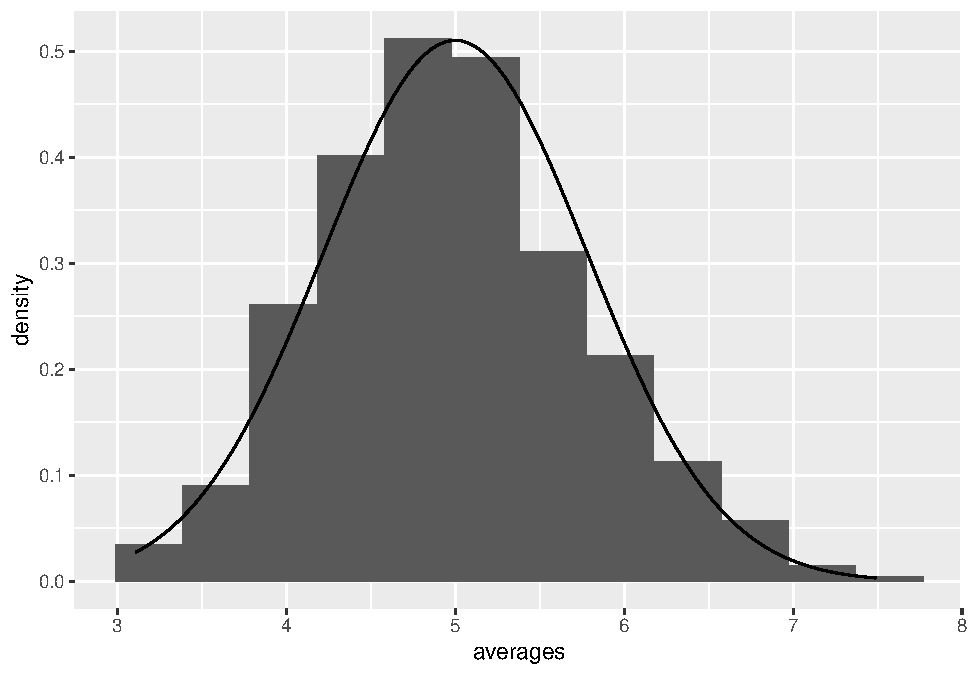
\includegraphics{Part1_files/figure-latex/unnamed-chunk-4-1.pdf} \#\# 4.
Evaluate the coverage.

Evaluate the coverage of the confidence interval for 1/lambda:
\[ \bar{X} \pm 1.96\frac{S}{\sqrt{n}}\].

\begin{Shaded}
\begin{Highlighting}[]
\KeywordTok{mean}\NormalTok{(averages) }\OperatorTok{+}\StringTok{ }\KeywordTok{c}\NormalTok{(}\OperatorTok{-}\DecValTok{1}\NormalTok{,}\DecValTok{1}\NormalTok{) }\OperatorTok{*}\StringTok{ }\FloatTok{1.96} \OperatorTok{*}\StringTok{ }\KeywordTok{sd}\NormalTok{(averages) }\OperatorTok{/}\StringTok{ }\KeywordTok{sqrt}\NormalTok{(}\KeywordTok{length}\NormalTok{(averages))}
\end{Highlighting}
\end{Shaded}

\begin{verbatim}
## [1] 4.941572 5.038478
\end{verbatim}


\end{document}
